% !TEX root = _yoko.tex

% ==========================================
% プロジェクト予稿（1P）の本文
% ==========================================

\section{はじめに}
音楽の演奏では，楽譜の再現に加え，演奏者が強弱やテンポの変化を加えることで豊かな表現を生み出すことが求められる．

しかし，演奏の事前段階において演奏表現を試行する機会が十分に確保されていない．

そこで本研究では，楽曲音源に演奏表現を挿入できるシステムの開発を行った．また，ロングトーン中にも演奏表現の付与を可能にした．これにより，楽曲に豊かな演奏表現を付与することが可能となる．


\section{システム概要}
\subsection{システム構成}
本システムの意図は，ユーザである楽器演奏者が実際に楽器を手に取り，演奏を行う前段階の状態で，演奏表現の検討をしてもらうことである．そのため，ユーザは全くの音楽初心者ではなく，ある程度，楽器演奏の機会がある人を対象者としてシステムの開発を行っている．

機能としては，MIDI音源を入力都市，強弱による演奏表現の付与が可能なシステムである．表現を付与したものは新たなMIDIファイルで出力される仕組みになっている．

また，システムの作成において，フレーズ内の演奏表現に関しては保科理論\cite{Hoshina98}を，システム自体は「Mixtract」\cite{mixtract}を参考に作成した．
\subsection{ロングトーンの表現}
先行研究での強弱表現では，音符ごとのVelocityという，音を発するアタックの強弱のパラメータで音量を制御している．そのため，ロングトーン中の演奏表現については考慮されていない．特に，鍵盤演奏においては音価を持続させようとすると，いつか音が減衰してしまう．

一方，対象の楽器が管楽器だとすると，息での強弱変化が可能なため，音を持続しているロングトーンの最中でも，音量を自在に変化させることが可能である．そのため，必ずしも音符単位で頂点が決まるのではなく，ロングトーンの途中でもフレーズの頂点を置くことが可能であるといえる．

本システムでは，Expressionという，拍よりさらに詳細な単位で強弱を制御可能なパラメータを用い，フレーズ内の音量変化を滑らかに補間することで，持続音系楽器の特性に即した表現を可能にした．
\subsection{フレーズ・頂点の決定}
フレーズの強弱表現を決めるため，ユーザは，開始小節・拍数，終了小節・拍数，頂点の小節・拍数，開始・頂点・終了地点でのExpression値を入力する．
これにより，単調な音量変化ではなく，より自然な抑揚を持つ演奏表現を再現できる．

指定された情報に基づき，システムはExpressionの挿入を行う．

\section{適用事例}
本システムの検証として，J.S.Bachの「フーガト短調 BWV 578」\cite{Bach}を用いて実装した．
選曲理由としては，テンポが遅めであり音量の変化が明確化されやすいためである．
また実装する音源は，単旋律の譜表で構成されたMIDIデータを作成した．原曲は鍵盤楽器のため，１段の譜表で複数旋律存在しており，強弱表現を付与した際に違いが不明瞭になると考えたからである．
オーボエ・B♭クラリネット・アルトクラリネット・ファゴットの4パートに編曲し，各パートに対して強弱表現を適用した．フレーズごとにExpression値を補完し，持続音の自然な音量変化を再現した．

以下は適用例（オーボエ）と，\ref{fig:yoko} は適用楽曲の譜面である．

・フレーズA：１小節１拍目～２小節４拍目

・フレーズB：３小節１拍目～３小節４拍目

\begin{figure}[tb]
	\centering
	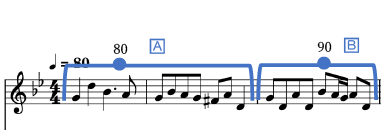
\includegraphics[width=\hsize]{fig/yoko.png}
	\caption{フレーズでの強弱を施したオーボエの譜面}
	\label{fig:yoko}
\end{figure}

結果として，鍵盤楽器向けのMIDI制御では不可能であった，ロングトーンの途中での強弱表現が可能となった．

\section{おわりに}
本研究では，持続音系楽器のための演奏表現付け支援システムを開発し，特にロングトーンの強弱変化に着目した手法を提案した．
今後はフレーズの自動解析機能の追加やGUIでの構築を行えば，システムの利便性はより高まるだろう．
